% Source: Graph_ML/Harmonic_Functions/harmonic_functions_on_graphs.tex
\begin{notechapter}
% ---- chapter-local definitions ----
\forgetcs\R\newcommand{\R}{\mathbb{R}}
\forgetcs\E\newcommand{\E}{\mathbb{E}}
\forgetcs\norm\newcommand{\norm}[1]{\left\|#1\right\|}
\forgetcs\abs\newcommand{\abs}[1]{\left|#1\right|}
\forgetcs\inner\newcommand{\inner}[2]{\langle #1, #2 \rangle}
\forgetcs\tr\newcommand{\tr}{\operatorname{tr}}
\forgetcs\diag\newcommand{\diag}{\operatorname{diag}}
\forgetcs\Area\newcommand{\Area}{\operatorname{Area}}
\forgetcs\Vol\newcommand{\Vol}{\operatorname{Vol}}
\definecolor{intuition}{RGB}{230,242,255}
\definecolor{examplecol}{RGB}{255,249,230}
\definecolor{connection}{RGB}{232,245,233}
\definecolor{warning}{RGB}{255,235,235}
\forgetenv{intuitionbox}\newtcolorbox{intuitionbox}[1][]{colback=intuition, 
  colframe=blue!50!black, title=Intuition, breakable, #1}
\forgetenv{examplebox}\newtcolorbox{examplebox}[1][]{colback=examplecol, 
  colframe=orange!50!black, title=Worked Example, breakable, #1}
\forgetenv{connectionbox}\newtcolorbox{connectionbox}[1][]{colback=connection, 
  colframe=green!50!black, title=Key Connection, breakable, #1}
\forgetenv{warningbox}\newtcolorbox{warningbox}[1][]{colback=warning,
  colframe=red!50!black, title=Caution, breakable, #1}
% -----------------------------------
\chapter{From Harmonic Functions to Graph Laplacians}\label{ch:harmonic-functions}
\chaptersubtitle{A unified perspective}

\begin{abstract}
This document explores the deep connection between classical harmonic
functions in continuous mathematics and their discrete analogues on graphs.
Starting from the one-dimensional case that every calculus student knows, we
build up to the Laplacian in $\R^d$ and derive its interpretation as a
measure of deviation from local averages. We then show how the graph
Laplacian emerges naturally as the discrete counterpart, and explain why
label propagation on graphs solves a discrete boundary value problem. The
presentation is self-contained, aimed at upper-undergraduate students, and
emphasizes worked examples and physical intuition alongside mathematical
rigor.
\end{abstract}

% ====================================================================
\section{Introduction}
% ====================================================================

Imagine you are holding a thin metal plate by its edges, and you heat some
edges to $100^\circ$C while cooling others to $0^\circ$C. After a long time,
the plate reaches a \emph{steady state}: the temperature at every interior
point stops changing. What determines this equilibrium temperature?

The answer, known since the work of Laplace in the 18th century, is that the
steady-state temperature is a \textbf{harmonic function}: at every interior
point, the temperature equals the average of the temperatures in a small
neighborhood around it. There are no ``hot spots'' or ``cold spots'' in the
interior---only a smooth interpolation between the boundary temperatures.

This same principle appears throughout mathematics and physics:
\begin{itemize}
    \item In \textbf{electrostatics}, the electric potential in a charge-free
          region is harmonic.
    \item In \textbf{heat transfer}, steady-state temperature distributions
          are harmonic.
    \item In \textbf{probability}, the expected value of a random walk at its
          stopping time is a harmonic function of the starting point.
\end{itemize}

Perhaps surprisingly, the same concept appears in \textbf{graph-based
machine learning}. When we run a label propagation algorithm on a
graph---assigning labels to unknown nodes based on the labels of their
neighbors---we are solving the \emph{discrete} analogue of the boundary
value problem that governs heat flow.

This document makes the connection precise. We start with the simplest
case (one dimension), build up to the general continuous theory, then show
how every key idea has an exact discrete counterpart on graphs.

\begin{connectionbox}[title=Roadmap]
\begin{enumerate}
    \item \textbf{Section~\ref{harmonic-functions:sec:1d}}: The one-dimensional case---harmonic
          functions are linear (familiar from calculus).
    \item \textbf{Section~\ref{harmonic-functions:sec:continuous}}: The Laplacian in $\R^d$ and
          the mean value property.
    \item \textbf{Section~\ref{harmonic-functions:sec:graph_laplacian}}: The graph Laplacian as
          the discrete analogue.
    \item \textbf{Section~\ref{harmonic-functions:sec:dirichlet}}: Boundary value problems,
          continuous and discrete.
    \item \textbf{Section~\ref{harmonic-functions:sec:random_walks}}: The random walk
          interpretation.
    \item \textbf{Section~\ref{harmonic-functions:sec:summary}}: The unifying principle.
\end{enumerate}
\end{connectionbox}


% ====================================================================
\section{Warm-Up: The One-Dimensional Case}
\label{harmonic-functions:sec:1d}
% ====================================================================

Before tackling multiple dimensions, let us start with the case every
calculus student knows.

\subsection{Harmonic Functions on \texorpdfstring{$\R$}{R}}

In one dimension, the Laplacian of a twice-differentiable function
$f : \R \to \R$ is simply its second derivative:
\begin{equation}
\Delta f(x) = f''(x)
\end{equation}
A function is \textbf{harmonic} on an interval $(a,b)$ if $f''(x) = 0$ for
all $x \in (a,b)$. Integrating twice, this means $f(x) = \alpha x + \beta$
for some constants $\alpha, \beta$: \emph{harmonic functions in one dimension
are exactly the linear functions.}

\subsection{The Mean Value Property in 1D}

Why do we say harmonic functions ``equal the average of their neighbors''?
In one dimension, the ``sphere of radius $r$ around $x$'' consists of just
two points: $x - r$ and $x + r$. The average over this sphere is:
\begin{equation}
\text{Average} = \frac{f(x-r) + f(x+r)}{2}
\end{equation}

If $f$ is linear, say $f(x) = \alpha x + \beta$, then:
\[
\frac{f(x-r) + f(x+r)}{2}
= \frac{(\alpha(x-r) + \beta) + (\alpha(x+r) + \beta)}{2}
= \alpha x + \beta = f(x)
\]
So a linear function equals the average of its values at $x \pm r$ for
\emph{every} $r$. This is the mean value property.

\subsection{The Laplacian Measures Deviation from the Average}

What if $f$ is \emph{not} harmonic? The second derivative measures exactly
how much $f(x)$ deviates from the average of its neighbors. To see this,
start from the Taylor expansions of $f(x+r)$ and $f(x-r)$ around $x$:
\begin{align}
f(x+r) &= f(x) + r\,f'(x) + \frac{r^2}{2}\,f''(x) + O(r^3) \\
f(x-r) &= f(x) - r\,f'(x) + \frac{r^2}{2}\,f''(x) + O(r^3)
\end{align}
Adding these two equations, the first-order terms cancel (they have opposite
signs), giving:
\begin{equation}
f(x+r) + f(x-r) = 2f(x) + r^2\,f''(x) + O(r^3)
\end{equation}
Rearranging and dividing by $r^2$:

\begin{equation}
\label{harmonic-functions:eq:1d_laplacian_avg}
f''(x) = \lim_{r \to 0} \frac{f(x-r) - 2f(x) + f(x+r)}{r^2}
= \lim_{r \to 0} \frac{2}{r^2}\left(
  \underbrace{\frac{f(x-r) + f(x+r)}{2}}_{\text{average of neighbors}}
  - f(x)\right)
\end{equation}

This is the \textbf{centered finite difference} formula for $f''(x)$.
It says:
\begin{itemize}
    \item $f''(x) > 0$: $f(x)$ is \emph{below} the average of its
          neighbors---the function is locally convex (like a valley).
    \item $f''(x) < 0$: $f(x)$ is \emph{above} the average of its
          neighbors---the function is locally concave (like a hilltop).
    \item $f''(x) = 0$: $f(x)$ \emph{equals} the average of its
          neighbors---the function is locally linear (harmonic).
\end{itemize}

\begin{examplebox}[title=The 1D Boundary Value Problem]
Consider a rod of length $L$ with temperature $T = 100^\circ$C at $x = 0$
and $T = 0^\circ$C at $x = L$. The steady-state temperature satisfies
$T''(x) = 0$ with boundary conditions $T(0) = 100$ and $T(L) = 0$. The
unique solution is:
\[
T(x) = 100\left(1 - \frac{x}{L}\right)
\]
A linear interpolation between the boundary values---exactly as the mean
value property predicts. At every interior point, the temperature equals
the average of its two neighbors.
\end{examplebox}

\begin{intuitionbox}
Formula~\eqref{harmonic-functions:eq:1d_laplacian_avg} is the key insight of this entire
document. The rest is about generalizing it: from one dimension to
$\R^d$ (Section~\ref{harmonic-functions:sec:continuous}), and from $\R^d$ to graphs
(Section~\ref{harmonic-functions:sec:graph_laplacian}). In every case, the Laplacian
measures the deviation of a function's value from the average of its
neighborhood.
\end{intuitionbox}


% ====================================================================
\section{The Laplacian and Mean Value Property in \texorpdfstring{$\R^d$}{Rd}}
\label{harmonic-functions:sec:continuous}
% ====================================================================

We now generalize the one-dimensional picture to higher dimensions.

\subsection{The Laplacian in Higher Dimensions}

\begin{definition}[Laplacian in $\R^d$]
\label{harmonic-functions:def:cont_laplacian}
For a twice-differentiable function $f: \R^d \to \R$, the \textbf{Laplacian}
is the sum of all unmixed second partial derivatives:
\begin{equation}
\Delta f = \frac{\partial^2 f}{\partial x_1^2}
         + \frac{\partial^2 f}{\partial x_2^2}
         + \cdots
         + \frac{\partial^2 f}{\partial x_d^2}
         = \tr(H_f)
\end{equation}
where $H_f$ is the Hessian matrix of $f$ (the $d \times d$ matrix of second
partial derivatives, $(H_f)_{ij} = \frac{\partial^2 f}{\partial x_i
\partial x_j}$), and $\tr$ denotes the trace.
\end{definition}

In one dimension, $\Delta f = f''$. In two dimensions,
$\Delta f = f_{xx} + f_{yy}$. Each term $\frac{\partial^2 f}{\partial x_k^2}$
measures the concavity of $f$ along the $x_k$-axis, and the Laplacian sums
these concavities over all coordinate directions.

\begin{definition}[Harmonic Function]
\label{harmonic-functions:def:harmonic_cont}
A function $f: \R^d \to \R$ is \textbf{harmonic} on a domain
$\Omega \subset \R^d$ if $\Delta f(x) = 0$ for all $x \in \Omega$.
\end{definition}

\begin{example}[Harmonic Functions]
\label{harmonic-functions:ex:harmonic_examples}
\leavevmode
\begin{itemize}
    \item \textbf{1D}: $f(x) = ax + b$ (all linear functions).
    \item \textbf{2D}: $f(x,y) = x^2 - y^2$ is harmonic because
          $f_{xx} = 2$ and $f_{yy} = -2$, so $\Delta f = 2 + (-2) = 0$.
          More examples: $f(x,y) = e^x \sin y$ and
          $f(x,y) = \ln(x^2 + y^2)$ (away from the origin).
    \item \textbf{3D}: The Coulomb potential
          $f(x,y,z) = 1/\sqrt{x^2 + y^2 + z^2}$ is harmonic away from the
          origin (the potential of a point charge satisfies Laplace's
          equation in the charge-free region).
\end{itemize}
\end{example}

\subsection{The Laplacian Measures Deviation from Local Averages}

In 1D, we saw that $f''(x)$ measures how much $f(x)$ deviates from the
average of $f(x-r)$ and $f(x+r)$. The same principle holds in any
dimension---but now the ``two neighbors at distance $r$'' are replaced by
the entire \emph{sphere} of radius $r$ around $x$.

We write $S^{d-1} = \{\mathbf{u} \in \R^d : \|\mathbf{u}\| = 1\}$ for the
unit sphere in $\R^d$ (it is $(d{-}1)$-dimensional: $S^0 = \{-1,+1\}$ in
$\R^1$, $S^1$ is the unit circle in $\R^2$, $S^2$ is the familiar sphere in
$\R^3$). For a point $x \in \R^d$ and radius $r > 0$, we write
$\partial B(x,r) = \{y \in \R^d : \|y - x\| = r\}$ for the sphere of
radius $r$ centered at $x$, and $\omega_{d-1} = \Area(S^{d-1})$ for the
surface area of the unit sphere.

\begin{definition}[Spherical Mean]
\label{harmonic-functions:def:spherical_mean}
For a function $f : \R^d \to \R$, the \textbf{spherical mean} of $f$ at
center $x$ with radius $r > 0$ is the average of $f$ over the sphere
$\partial B(x,r)$:
\begin{equation}
M_f(x, r) = \frac{1}{\omega_{d-1}\,r^{d-1}}
  \int_{\partial B(x,r)} f(y)\,d\sigma(y)
\end{equation}
where $d\sigma$ denotes the surface area element on the sphere. The
denominator $\omega_{d-1}\,r^{d-1} = \Area(\partial B(x,r))$ is the total
surface area of the sphere of radius $r$.
\end{definition}

In 1D, $\partial B(x,r) = \{x-r,\, x+r\}$ and
$M_f(x,r) = \frac{f(x-r) + f(x+r)}{2}$: the spherical mean reduces to
the average of the two neighbors, recovering the formula from
Section~\ref{harmonic-functions:sec:1d}. In 2D, it is the average of $f$ around a circle; in
3D, the average over a sphere.

\begin{theorem}[Laplacian as Deviation from Spherical Mean]
\label{harmonic-functions:thm:laplacian_average}
For a smooth function $f: \R^d \to \R$:
\begin{equation}
\label{harmonic-functions:eq:laplacian_avg}
\boxed{\Delta f(x) = \lim_{r \to 0} \frac{2d}{r^2}
  \bigl(M_f(x,r) - f(x)\bigr)}
\end{equation}
Equivalently, the spherical mean admits the expansion:
\begin{equation}
\label{harmonic-functions:eq:spherical_mean_expansion}
M_f(x,r) = f(x) + \frac{r^2}{2d}\,\Delta f(x) + O(r^4)
\end{equation}
(The $O(r^3)$ term vanishes because odd-order terms integrate to zero on
the sphere by the same symmetry that killed the first-order term.)
\end{theorem}

Compare this with the 1D formula~\eqref{harmonic-functions:eq:1d_laplacian_avg}: the structure
is identical. The factor $2d/r^2$ generalizes the factor $2/r^2$ from 1D
(where $d = 1$). The average over the two-point ``sphere'' $\{x-r, x+r\}$
is replaced by the average over the full $(d-1)$-dimensional sphere of
radius~$r$.

\begin{proof}
Let $y = x + r\mathbf{u}$ where $\mathbf{u}$ is a unit vector. Taylor expand
$f$ around $x$ to second order:
\begin{equation}
f(x + r\mathbf{u}) = f(x) + r\,\nabla f(x) \cdot \mathbf{u}
  + \frac{r^2}{2}\,\mathbf{u}^\top H_f(x)\,\mathbf{u} + O(r^3)
\end{equation}
Now average over all unit directions $\mathbf{u}$ on the sphere $S^{d-1}$.

\textbf{The zeroth-order term} $f(x)$ is constant and passes through the
average unchanged.

\textbf{The first-order term} $r\,\nabla f(x) \cdot \mathbf{u}$ vanishes
upon averaging. This is because for every direction $\mathbf{u}$, the
opposite direction $-\mathbf{u}$ appears with equal weight on the sphere,
and $\nabla f(x) \cdot (-\mathbf{u}) = -\nabla f(x) \cdot \mathbf{u}$. So
the contributions cancel in pairs:
\[
\frac{1}{\Area(S^{d-1})} \int_{S^{d-1}}
  \nabla f(x) \cdot \mathbf{u}\,dS(\mathbf{u}) = 0
\]

\textbf{The second-order term} is the interesting one. We need to compute:
\[
\frac{1}{\Area(S^{d-1})} \int_{S^{d-1}}
  \mathbf{u}^\top H_f(x)\,\mathbf{u}\,dS(\mathbf{u})
\]

\begin{lemma}[Spherical Average of a Quadratic Form]
\label{harmonic-functions:lem:sphere_average_quadratic}
For any symmetric matrix $H \in \R^{d \times d}$:
\begin{equation}
\frac{1}{\Area(S^{d-1})} \int_{S^{d-1}}
  \mathbf{u}^\top H\,\mathbf{u}\,dS(\mathbf{u}) = \frac{1}{d}\,\tr(H)
\end{equation}
\end{lemma}

In words: when you average the quadratic form $\mathbf{u}^\top H\mathbf{u}$
over all directions $\mathbf{u}$ on the unit sphere, you get $\tr(H)/d$
regardless of the off-diagonal structure of $H$. Only the diagonal (the
trace) survives the averaging---all directional biases wash out.

\begin{proof}[Proof of Lemma]
The proof has three steps.

\textbf{Step 1: Expand using the eigenbasis.} Since $H$ is a real symmetric
matrix, the spectral theorem guarantees that it has $d$ real eigenvalues
$\lambda_1, \ldots, \lambda_d$ and an orthonormal eigenbasis
$\mathbf{v}_1, \ldots, \mathbf{v}_d$. We can write:
\[
H = \sum_{i=1}^d \lambda_i\,\mathbf{v}_i\mathbf{v}_i^\top
\]
Substituting into the quadratic form:
\[
\mathbf{u}^\top H\,\mathbf{u}
= \sum_{i=1}^d \lambda_i\,
  (\mathbf{v}_i^\top\mathbf{u})(\mathbf{v}_i^\top\mathbf{u})
= \sum_{i=1}^d \lambda_i\,(\mathbf{v}_i \cdot \mathbf{u})^2
\]
Here $\mathbf{v}_i \cdot \mathbf{u}$ is the component of $\mathbf{u}$ along
the $i$-th eigendirection. Integrating over the sphere:
\begin{equation}
\label{harmonic-functions:eq:quadratic_expansion}
\int_{S^{d-1}} \mathbf{u}^\top H\,\mathbf{u}\,dS(\mathbf{u})
= \sum_{i=1}^d \lambda_i
  \underbrace{\int_{S^{d-1}}(\mathbf{v}_i \cdot \mathbf{u})^2\,
  dS(\mathbf{u})}_{=:\, I_i}
\end{equation}

\textbf{Step 2: Symmetry argument---all $I_i$ are equal.} The integral $I_i$
asks: ``how much does a random direction on the sphere align with the fixed
direction $\mathbf{v}_i$?'' But the sphere has no preferred direction---it
looks the same from every angle. Formally, for any rotation $R$ that maps
$\mathbf{v}_i$ to $\mathbf{v}_j$, the change of variables
$\mathbf{u} \mapsto R\mathbf{u}$ leaves the sphere and its surface measure
invariant, so $I_i = I_j$. All $d$ integrals equal the same constant:
$I_1 = I_2 = \cdots = I_d =: C$.

\textbf{Step 3: Compute $C$ by summing over all directions.} Since
$\{\mathbf{v}_1, \ldots, \mathbf{v}_d\}$ is an orthonormal basis, every
unit vector $\mathbf{u}$ can be decomposed as
$\mathbf{u} = \sum_{i=1}^d (\mathbf{v}_i \cdot \mathbf{u})\,\mathbf{v}_i$,
and by Parseval's identity:
\[
\sum_{i=1}^d (\mathbf{v}_i \cdot \mathbf{u})^2 = \|\mathbf{u}\|^2 = 1
\quad\text{for every } \mathbf{u} \in S^{d-1}
\]
Integrating both sides over the sphere:
\[
\sum_{i=1}^d I_i = \int_{S^{d-1}} 1\,dS(\mathbf{u}) = \Area(S^{d-1})
\]
Since all $I_i$ equal $C$: $\;d \cdot C = \Area(S^{d-1})$, giving
$C = \Area(S^{d-1})/d$.

\textbf{Conclusion.} We can now assemble the pieces. From
Step~1, equation~\eqref{harmonic-functions:eq:quadratic_expansion}:
\[
\int_{S^{d-1}} \mathbf{u}^\top H\,\mathbf{u}\,dS(\mathbf{u})
= \sum_{i=1}^d \lambda_i\, I_i
\]
From Step~2, each $I_i$ equals the same constant $C$. From Step~3,
$C = \Area(S^{d-1})/d$. Substituting:
\[
\sum_{i=1}^d \lambda_i\, I_i
= \sum_{i=1}^d \lambda_i \cdot C
= C \sum_{i=1}^d \lambda_i
= \frac{\Area(S^{d-1})}{d}\sum_{i=1}^d \lambda_i
\]
Finally, the sum of the eigenvalues equals the trace. To see this, recall
that the trace is invariant under cyclic permutations:
$\tr(ABC) = \tr(CAB)$. Applying this to the eigendecomposition
$H = Q\Lambda Q^\top$ (where $Q$ is orthogonal and $\Lambda = \diag(\lambda_1, \ldots, \lambda_d)$):
\[
\tr(H) = \tr(Q\Lambda Q^\top) = \tr(Q^\top Q\Lambda)
= \tr(I \cdot \Lambda) = \tr(\Lambda) = \sum_{i=1}^d \lambda_i
\]
So:
\[
\int_{S^{d-1}} \mathbf{u}^\top H\,\mathbf{u}\,dS(\mathbf{u})
= \frac{\Area(S^{d-1})}{d}\,\tr(H)
\]
Dividing both sides by $\Area(S^{d-1})$ gives the result.
\end{proof}

\begin{examplebox}[title=Verifying the Lemma in 2D]
In $\R^2$, the unit sphere $S^1$ is the unit circle, parametrized by
$\mathbf{u} = (\cos\theta, \sin\theta)$ for $\theta \in [0, 2\pi)$, with
$\Area(S^1) = 2\pi$.

Take $H = \begin{psmallmatrix} 3 & 1 \\ 1 & 5 \end{psmallmatrix}$, which
has $\tr(H) = 8$. The lemma predicts:
\[
\frac{1}{2\pi}\int_0^{2\pi}
  \mathbf{u}^\top H\,\mathbf{u}\,d\theta
= \frac{\tr(H)}{d} = \frac{8}{2} = 4
\]

Let us verify by direct computation. Expanding
$\mathbf{u}^\top H\,\mathbf{u}$:
\begin{align}
\mathbf{u}^\top H\,\mathbf{u}
&= 3\cos^2\theta + 2\cos\theta\sin\theta + 5\sin^2\theta \\
&= 3\cdot\tfrac{1+\cos 2\theta}{2}
 + \sin 2\theta
 + 5\cdot\tfrac{1-\cos 2\theta}{2} \\
&= 4 - \cos 2\theta + \sin 2\theta
\end{align}
Averaging over $[0, 2\pi)$: the $\cos 2\theta$ and $\sin 2\theta$ terms
integrate to zero, leaving exactly $4$. \checkmark

Note how the off-diagonal entry ($H_{12} = 1$) contributed the
$\sin 2\theta$ term, which vanishes upon averaging. The diagonal entries
contributed $\frac{3+5}{2} = 4 = \tr(H)/d$. This is the general
phenomenon: averaging over all directions kills everything except the trace.
\end{examplebox}

\begin{examplebox}[title=Verifying the Lemma in 3D]
In $\R^3$, we use a diagonal matrix for simplicity. Take
$H = \diag(2, 5, 8)$, so $\tr(H) = 15$. The lemma predicts:
\[
\frac{1}{\Area(S^2)}\int_{S^2}
  \mathbf{u}^\top H\,\mathbf{u}\,dS(\mathbf{u})
= \frac{15}{3} = 5
\]

Parametrize the unit sphere with spherical coordinates:
$\mathbf{u} = (\sin\phi\cos\theta,\;\sin\phi\sin\theta,\;\cos\phi)$
where $\phi \in [0,\pi]$ and $\theta \in [0,2\pi)$, with surface element
$dS = \sin\phi\,d\phi\,d\theta$. Since $H$ is diagonal:
\[
\mathbf{u}^\top H\,\mathbf{u}
= 2\sin^2\!\phi\cos^2\!\theta
+ 5\sin^2\!\phi\sin^2\!\theta
+ 8\cos^2\!\phi
\]

We use the standard spherical integrals (which follow from
$\int_0^{2\pi}\cos^2\!\theta\,d\theta
= \int_0^{2\pi}\sin^2\!\theta\,d\theta = \pi$ and
$\int_0^{\pi}\sin^3\!\phi\,d\phi = 4/3$,
$\int_0^{\pi}\cos^2\!\phi\sin\phi\,d\phi = 2/3$):
\begin{align}
\int_{S^2}\sin^2\!\phi\cos^2\!\theta\,dS
&= \pi \cdot \tfrac{4}{3} = \tfrac{4\pi}{3} \\
\int_{S^2}\sin^2\!\phi\sin^2\!\theta\,dS
&= \pi \cdot \tfrac{4}{3} = \tfrac{4\pi}{3} \\
\int_{S^2}\cos^2\!\phi\,dS
&= 2\pi \cdot \tfrac{2}{3} = \tfrac{4\pi}{3}
\end{align}
All three integrals equal $4\pi/3 = \Area(S^2)/3$, confirming the symmetry
argument: each coordinate direction captures the same fraction $1/d = 1/3$
of the total surface area $\Area(S^2) = 4\pi$. Therefore:
\[
\int_{S^2} \mathbf{u}^\top H\,\mathbf{u}\,dS
= 2 \cdot \tfrac{4\pi}{3} + 5 \cdot \tfrac{4\pi}{3}
  + 8 \cdot \tfrac{4\pi}{3}
= \tfrac{4\pi}{3}(2 + 5 + 8)
= \tfrac{4\pi}{3}\cdot 15 = 20\pi
\]
Dividing by $\Area(S^2) = 4\pi$: the average is $20\pi / 4\pi = 5 =
\tr(H)/3$. \checkmark
\end{examplebox}

\medskip
\noindent\textbf{Returning to the proof of
Theorem~\ref{harmonic-functions:thm:laplacian_average}.} We left the main proof at the point
where we needed to evaluate the second-order term in the Taylor expansion of
$M_f(x,r)$. That term involved the spherical average of
$\mathbf{u}^\top H_f(x)\,\mathbf{u}$---exactly the quantity that
Lemma~\ref{harmonic-functions:lem:sphere_average_quadratic} computes. We now apply it with
$H = H_f(x)$ (the Hessian of $f$ at $x$), for which
$\tr(H_f(x)) = \Delta f(x)$ (by Definition~\ref{harmonic-functions:def:cont_laplacian}).

Combining the zeroth-order term $f(x)$, the vanishing first-order term, and
the second-order term evaluated by the lemma:
\begin{align}
M_f(x,r)
&= \frac{1}{\Area(S^{d-1})} \int_{S^{d-1}}
   f(x + r\mathbf{u})\,dS(\mathbf{u}) \\
&= f(x) + \underbrace{0}_{\text{1st order}}
   + \frac{r^2}{2}\cdot
   \underbrace{\frac{1}{d}\,\tr(H_f(x))}_{\text{Lemma~\ref{harmonic-functions:lem:sphere_average_quadratic}}}
   + O(r^4) \\
&= f(x) + \frac{r^2}{2d}\,\Delta f(x) + O(r^4)
\end{align}
(The $O(r^3)$ term vanishes because the third-order Taylor contribution
$r^3 \sum_{ijk} \partial_{ijk}f\, u_i u_j u_k$ is an odd function of
$\mathbf{u}$ and integrates to zero on the sphere, just like the first-order
term did.)

Rearranging:
\[
\frac{2d}{r^2}\bigl(M_f(x,r) - f(x)\bigr)
= \Delta f(x) + O(r^2)
\]
Taking $r \to 0$ yields the result.
\end{proof}

\subsection{The Mean Value Property}

Let us recall what the spherical mean expansion~\eqref{harmonic-functions:eq:spherical_mean_expansion} tells us for a smooth function:
\[
M_f(x,r) = f(x) + \frac{r^2}{2d}\,\Delta f(x) + O(r^4)
\]
When $f$ is harmonic ($\Delta f = 0$), the $r^2$ term vanishes, so
$M_f(x,r) = f(x) + O(r^4)$: the spherical mean equals $f(x)$ up to a
small error for small $r$. But one might wonder: does the $O(r^4)$
remainder also vanish, or is there still a discrepancy at finite radius?

The answer is striking: \emph{the equality is exact for every radius}, with
no error term at all.

\begin{theorem}[Mean Value Property]
\label{harmonic-functions:thm:mean_value}
If $f$ is harmonic on a domain $\Omega \subset \R^d$, then for any point
$x \in \Omega$ and any radius $r > 0$ such that the closed ball
$\overline{B(x,r)} \subset \Omega$:
\begin{equation}
M_f(x,r) = f(x)
\end{equation}
The value of $f$ at the center equals the spherical mean for every
radius---with no error term and no limit.
\end{theorem}

\begin{proof}[Proof sketch]
Consider $M_f(x,r)$ as a function of $r$ alone. A computation using the
divergence theorem shows that:
\[
\frac{d}{dr}M_f(x,r)
= \frac{r}{d}\,\frac{1}{\omega_{d-1}\,r^{d-1}}
  \int_{B(x,r)} \Delta f(y)\,dV(y)
\]
When $\Delta f = 0$ throughout $\Omega$, the integrand vanishes, so
$\frac{d}{dr}M_f(x,r) = 0$ for all admissible $r$. This means $M_f(x,r)$
is constant in $r$, and its value is $\lim_{r \to 0^+} M_f(x,r) = f(x)$.
\end{proof}

This theorem is the higher-dimensional generalization of the 1D observation
from Section~\ref{harmonic-functions:sec:1d}: a linear function on $\R$ equals the average of
its values at $x - r$ and $x + r$ for every $r$, not just in the limit. The
mean value property is the defining characteristic of harmonic functions,
and it is precisely this property that label propagation reproduces on
graphs (Section~\ref{harmonic-functions:sec:graph_laplacian}).

\begin{intuitionbox}
\textbf{Physical interpretation of the Laplacian:}
\begin{itemize}
    \item $\Delta f(x) > 0$: $f(x)$ is \emph{below} the local average
          (like a valley). In heat flow, heat flows \emph{in}---the point
          warms up.
    \item $\Delta f(x) < 0$: $f(x)$ is \emph{above} the local average
          (like a hilltop). Heat flows \emph{out}---the point cools down.
    \item $\Delta f(x) = 0$: $f(x)$ \emph{equals} the local average. No
          net heat flow---the system is in equilibrium. This is the
          harmonic condition.
\end{itemize}
\end{intuitionbox}

\begin{examplebox}[title=Verifying the Mean Value Property in 2D]
Consider $f(x,y) = x^2 - y^2$, which is harmonic ($\Delta f = 2 - 2 = 0$).
Take the point $(0,0)$ where $f(0,0) = 0$. On the circle of radius $r$,
parametrize as $(x,y) = (r\cos\theta,\, r\sin\theta)$:
\[
\frac{1}{2\pi} \int_0^{2\pi} f(r\cos\theta, r\sin\theta)\,d\theta
= \frac{r^2}{2\pi} \int_0^{2\pi} (\cos^2\theta - \sin^2\theta)\,d\theta
= \frac{r^2}{2\pi} \int_0^{2\pi} \cos 2\theta\,d\theta = 0 = f(0,0)
\]
The average over the circle equals the value at the center, as predicted.
\end{examplebox}


% ====================================================================
\section{Discrete Analogue: The Graph Laplacian}
\label{harmonic-functions:sec:graph_laplacian}
% ====================================================================

We now move from continuous domains to graphs. The transition is guided by a
single principle: \emph{replace the spherical average with the neighborhood
average}.

Consider a \textbf{connected} undirected weighted graph $G = (V, E, A)$ with
$n$ nodes, adjacency matrix $A$ (where $A_{ij} \geq 0$ is the weight of edge
$\{i,j\}$), and degree matrix $D = \diag(d_1, \ldots, d_n)$ where
$d_i = \sum_j A_{ij}$. Connectivity means that every pair of nodes is linked
by some path---the graph analogue of a connected domain $\Omega$ in the
continuous setting. A function on the graph is simply a vector
$f \in \R^n$, with $f_i$ being the value at node $v_i$.

\subsection{From Continuous to Discrete: The Key Substitution}

In the continuous world, the Laplacian measures the deviation of $f(x)$ from
its spherical average. On a graph, the ``sphere around node $v_i$'' is
naturally replaced by the \textbf{neighborhood} $\mathcal{N}(i)$, and the
spherical average becomes the \textbf{weighted average over neighbors}:
\begin{equation}
\text{Average over neighbors of } v_i
= \frac{1}{d_i}\sum_{j} A_{ij}\,f_j
= \sum_j P_{ij}\,f_j
\end{equation}
where $P = D^{-1}A$ is the random walk transition matrix (the entry $P_{ij}
= A_{ij}/d_i$ is the probability that a random walker at $v_i$ moves to
$v_j$).

This substitution leads directly to the graph Laplacian.

\subsection{The Random Walk Laplacian}

\begin{definition}[Random Walk Laplacian]
\label{harmonic-functions:def:rw_laplacian}
The \textbf{random walk Laplacian} is $\mathcal{L}_{\mathrm{rw}} = I - P
= I - D^{-1}A$. Its action on a function $f$ is:
\begin{equation}
(\mathcal{L}_{\mathrm{rw}} f)_i
= f_i - \sum_j P_{ij}\,f_j
= \underbrace{f_i\vphantom{\sum_j}}_{\mathclap{\substack{\text{value}\\
  \text{at node}}}}
  - \quad \underbrace{\sum_j P_{ij}\,f_j}_{\mathclap{\substack{
  \text{weighted average}\\ \text{of neighbors}}}}
\end{equation}
\end{definition}

This is the \emph{exact discrete counterpart} of the continuous Laplacian
formula from Theorem~\ref{harmonic-functions:thm:laplacian_average}: the value at a point minus
the average over its neighborhood. Compare:
\begin{align}
\text{Continuous:} &\quad \Delta f(x) \propto
  \bigl(\text{average of $f$ on sphere}\bigr) - f(x) \\
\text{Graph:} &\quad (\mathcal{L}_{\mathrm{rw}} f)_i
  = f_i - \bigl(\text{average of $f$ over neighbors}\bigr)
\end{align}

\begin{warningbox}
Note the sign convention: in the continuous case, $\Delta f > 0$ means $f$
is below its local average, while $(\mathcal{L}_{\mathrm{rw}} f)_i > 0$
means $f_i$ is \emph{above} its neighbor average. This is because the graph
Laplacian is conventionally defined as $f_i - \text{avg}$ rather than
$\text{avg} - f_i$. Both conventions appear in the literature; the discrete
convention $\mathcal{L}_{\mathrm{rw}} = I - P$ is standard in graph
theory.
\end{warningbox}

\begin{definition}[Harmonic Function on a Graph]
\label{harmonic-functions:def:harmonic_graph}
A function $f: V \to \R$ is \textbf{harmonic at node $v_i$} if:
\begin{equation}
f_i = \sum_j P_{ij}\,f_j
\end{equation}
Equivalently, $(\mathcal{L}_{\mathrm{rw}} f)_i = 0$. A function is harmonic
on a set $S \subset V$ if it is harmonic at every node in $S$.
\end{definition}

Just as in the continuous case, a harmonic function on a graph has no local
extrema on the interior: no node's value can be strictly larger (or smaller)
than all its neighbors'. Every value is a weighted average---a compromise.

\subsection{The Unnormalized Laplacian}

There is a second, closely related graph Laplacian that is important in
spectral graph theory.

\begin{definition}[Unnormalized Laplacian]
\label{harmonic-functions:def:unnorm_laplacian}
The \textbf{unnormalized Laplacian} is $L = D - A$, with:
\begin{equation}
(Lf)_i = d_i\,f_i - \sum_j A_{ij}\,f_j
= d_i\left(f_i - \frac{1}{d_i}\sum_j A_{ij}\,f_j\right)
= d_i \cdot (\mathcal{L}_{\mathrm{rw}} f)_i
\end{equation}
\end{definition}

The unnormalized Laplacian is simply the random walk Laplacian scaled by the
degree: $(Lf)_i = d_i \cdot (\mathcal{L}_{\mathrm{rw}} f)_i$. The degree
$d_i$ plays the role of the factor $2d/r^2$ in the continuous
formula~\eqref{harmonic-functions:eq:laplacian_avg}---it accounts for the ``size'' of the
neighborhood.

The unnormalized Laplacian has a beautiful quadratic form that measures
the total variation of $f$ across edges:
\begin{equation}
\label{harmonic-functions:eq:laplacian_quadratic}
f^\top L f = \frac{1}{2}\sum_{i,j} A_{ij}(f_i - f_j)^2
\end{equation}
This is the discrete analogue of the Dirichlet energy
$\int_\Omega \|\nabla f\|^2\,dV$ from continuous PDE theory. Both measure
how much $f$ varies: a constant function has zero energy, and a rapidly
oscillating function has high energy.

\subsection{Worked Example: Harmonicity on a Small Graph}

\begin{examplebox}[title=A Weighted Triangle]
Consider a triangle with nodes $a$, $b$, $u$ and edge weights
$A_{au} = 1$, $A_{bu} = 2$, $A_{ab} = 3$. Fix $f_a = 1$ and
$f_b = 0$ (boundary). What value of $f_u$ makes $f$ harmonic at~$u$?

Node $u$ has degree $d_u = 1 + 2 = 3$, so $P_{ua} = 1/3$ and
$P_{ub} = 2/3$. The harmonic condition gives:
\[
f_u = P_{ua}\,f_a + P_{ub}\,f_b = \frac{1}{3}(1) + \frac{2}{3}(0)
= \frac{1}{3}
\]

The stronger edge to $b$ (weight 2) pulls $u$'s value closer to $f_b = 0$
than the weaker edge to $a$ (weight 1) pulls it toward $f_a = 1$.

We can verify: $(\mathcal{L}_{\mathrm{rw}} f)_u = f_u - (P_{ua}f_a +
P_{ub}f_b) = 1/3 - 1/3 = 0$ \checkmark.
\end{examplebox}

\begin{examplebox}[title=The Path Graph (Discrete Rod)]
Consider the path $v_1 - v_2 - v_3 - v_4 - v_5$ with $f_1 = 1$ and
$f_5 = 0$ (boundary nodes). Each interior node has two neighbors with
equal weight, so the harmonic condition becomes:
\begin{align}
f_2 &= \tfrac{1}{2}(f_1 + f_3) = \tfrac{1}{2}(1 + f_3) \\
f_3 &= \tfrac{1}{2}(f_2 + f_4) \\
f_4 &= \tfrac{1}{2}(f_3 + f_5) = \tfrac{1}{2}(f_3 + 0)
\end{align}
Solving this system (substitute from the outside in): $f_2 = 3/4$,
$f_3 = 1/2$, $f_4 = 1/4$.

\begin{center}
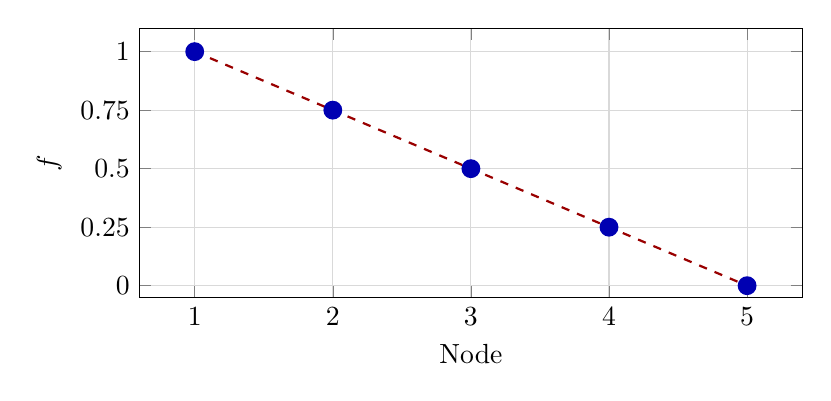
\begin{tikzpicture}[scale=1.0]
    \begin{axis}[
        width=10cm, height=5cm,
        xlabel={Node}, ylabel={$f$},
        xtick={1,2,3,4,5},
        ytick={0,0.25,0.5,0.75,1},
        ymin=-0.05, ymax=1.1,
        grid=major, grid style={gray!30},
        every axis plot/.style={thick}
    ]
    \addplot[only marks, mark=*, mark size=3pt, blue!70!black] coordinates
      {(1,1) (2,0.75) (3,0.5) (4,0.25) (5,0)};
    \addplot[dashed, red!60!black, domain=1:5] {1 - (x-1)/4};
    \end{axis}
\end{tikzpicture}
\end{center}

The discrete solution (blue dots) is a linear interpolation between the
boundary values---exactly the discrete analogue of the continuous 1D
harmonic function $T(x) = 1 - x/L$ from Section~\ref{harmonic-functions:sec:1d} (red dashed).
\end{examplebox}

\subsection{Summary of the Analogy}

\begin{connectionbox}[title=Continuous $\longleftrightarrow$ Discrete]
\begin{center}
\begin{tabular}{lll}
\toprule
\textbf{Continuous} & \textbf{Discrete (graph)} & \textbf{Interpretation} \\
\midrule
Sphere of radius $r$ & Neighborhood $\mathcal{N}(i)$ & Local region \\[3pt]
$\displaystyle\frac{1}{|\partial B|}
  \int_{\partial B}\!f\,dS$ &
$\displaystyle\frac{1}{d_i}\sum_j A_{ij}f_j$ & Local average \\[6pt]
$\Delta f(x) = 0$ & $(\mathcal{L}_{\mathrm{rw}} f)_i = 0$ &
  Harmonic condition \\[3pt]
$\displaystyle\int_\Omega \|\nabla f\|^2\,dV$ &
$\displaystyle\frac{1}{2}\sum_{i,j} A_{ij}(f_i - f_j)^2$ &
  Smoothness energy \\[3pt]
Dirichlet problem & Label propagation & Boundary value problem \\
\bottomrule
\end{tabular}
\end{center}
\end{connectionbox}


% ====================================================================
\section{The Dirichlet Problem: Continuous and Discrete}
\label{harmonic-functions:sec:dirichlet}
% ====================================================================

The connection becomes most powerful when we consider boundary value
problems---finding a function that is harmonic in the interior and matches
prescribed values on the boundary.

\subsection{The Continuous Dirichlet Problem}

\begin{definition}[Continuous Dirichlet Problem]
\label{harmonic-functions:def:cont_dirichlet}
Given a domain $\Omega \subset \R^d$ with boundary $\partial\Omega$, and a
function $g : \partial\Omega \to \R$ specifying boundary values, find
$f : \overline{\Omega} \to \R$ such that:
\begin{align}
\Delta f(x) &= 0 \quad \text{for } x \in \Omega
  \quad\text{(harmonic in the interior)} \\
f(x) &= g(x) \quad \text{for } x \in \partial\Omega
  \quad\text{(matches boundary values)}
\end{align}
\end{definition}

Under mild regularity conditions (the boundary $\partial\Omega$ is smooth
enough), this problem has a unique solution. The solution has several
equivalent characterizations:
\begin{enumerate}
    \item It is the unique function that is harmonic inside $\Omega$ and
          matches $g$ on the boundary.
    \item It minimizes the \textbf{Dirichlet energy}
          $\int_\Omega \|\nabla f\|^2\,dV$ among all functions that match
          $g$ on $\partial\Omega$. (The smoothest interpolation.)
    \item It satisfies the mean value property at every interior point.
    \item It can be computed via Brownian motion
          (Section~\ref{harmonic-functions:sec:random_walks}).
\end{enumerate}

\subsection{The Discrete Dirichlet Problem (Label Propagation)}

\begin{definition}[Discrete Dirichlet Problem on a Graph]
\label{harmonic-functions:def:graph_dirichlet}
Given a connected graph $G = (V, E, A)$, a set of \textbf{boundary nodes}
$\mathcal{V}_L \subset V$ with prescribed values $f_i = y_i$ for
$i \in \mathcal{V}_L$, find $f : V \to \R$ such that:
\begin{align}
(\mathcal{L}_{\mathrm{rw}} f)_i &= 0 \quad \text{for }
  i \in \mathcal{V}_U = V \setminus \mathcal{V}_L
  \quad\text{(harmonic on interior)} \\
f_i &= y_i \quad \text{for } i \in \mathcal{V}_L
  \quad\text{(boundary condition)}
\end{align}
\end{definition}

\begin{theorem}[Solution of the Discrete Dirichlet Problem]
\label{harmonic-functions:thm:discrete_dirichlet}
Let $G$ be connected with at least one boundary node. Then the discrete
Dirichlet problem has a unique solution given by:
\begin{equation}
f_U = (I - P_{UU})^{-1}\,P_{UL}\,f_L
\end{equation}
where $f_U$ and $f_L$ are the vectors of values at interior and boundary
nodes respectively, and the transition matrix $P$ is partitioned into blocks
according to the split $V = \mathcal{V}_U \cup \mathcal{V}_L$:
\begin{equation}
P = \begin{pmatrix} P_{UU} & P_{UL} \\ P_{LU} & P_{LL} \end{pmatrix}
\end{equation}
Here $P_{UU}$ contains transition probabilities between interior nodes,
$P_{UL}$ from interior nodes to boundary nodes, and so on.
\end{theorem}

\begin{proof}
The harmonic condition $f_i = \sum_j P_{ij}\,f_j$ at each interior node,
combined with the fixed boundary values, gives in block form:
\[
f_U = P_{UU}\,f_U + P_{UL}\,f_L
\]
Rearranging: $(I - P_{UU})\,f_U = P_{UL}\,f_L$. The matrix $I - P_{UU}$ is
invertible because $G$ is connected: the sub-matrix $P_{UU}$ is
sub-stochastic (its spectral radius is strictly less than~1, since a random
walk confined to $\mathcal{V}_U$ eventually escapes to a boundary node). The
full argument is given in Appendix~\ref{harmonic-functions:app:proof_dirichlet}.
\end{proof}

This is \emph{exactly} the label propagation algorithm: iteratively replace
each unlabeled node's value by the average of its neighbors' values (while
keeping boundary values fixed) until convergence. The iterative process
converges to the unique discrete harmonic function.

\subsection{Energy Minimization: The Discrete Dirichlet Energy}

Just as the continuous Dirichlet problem minimizes
$\int_\Omega \|\nabla f\|^2\,dV$, the discrete problem minimizes the graph
energy:

\begin{proposition}[Discrete Energy Minimization]
\label{harmonic-functions:prop:energy_min}
Among all functions $f : V \to \R$ that match the boundary values $y_i$
on $\mathcal{V}_L$, the discrete harmonic function uniquely minimizes:
\begin{equation}
E(f) = \frac{1}{2}\sum_{i,j} A_{ij}(f_i - f_j)^2 = f^\top L f
\end{equation}
\end{proposition}

\begin{proof}[Proof sketch]
The proof is a constrained optimization. Since only $f_U$ is free (the
boundary values $f_L$ are fixed), we differentiate $E(f)$ with respect to
$f_U$ and set the gradient to zero. This yields the harmonic condition
$(\mathcal{L}_{\mathrm{rw}} f)_i = 0$ on interior nodes. The full
derivation is in Appendix~\ref{harmonic-functions:app:proof_energy}.
\end{proof}

This gives a second way to understand label propagation: it finds the
\textbf{smoothest possible} assignment of values to unlabeled nodes, where
``smooth'' means that neighboring nodes have similar values. The boundary
values act as constraints, and the solution is the gentlest interpolation
through the graph.

\begin{center}
\begin{tabular}{ll}
\toprule
\textbf{Continuous} & \textbf{Discrete} \\
\midrule
$\displaystyle E(f) = \int_\Omega \|\nabla f\|^2\,dV$ &
$\displaystyle E(f) = \frac{1}{2}\sum_{i,j} A_{ij}(f_i - f_j)^2$ \\[6pt]
Euler--Lagrange: $\Delta f = 0$ &
Optimality: $(\mathcal{L}_{\mathrm{rw}} f)_i = 0$ on interior \\
\bottomrule
\end{tabular}
\end{center}


% ====================================================================
\section{Random Walk Interpretation}
\label{harmonic-functions:sec:random_walks}
% ====================================================================

The deepest connection between continuous and discrete harmonic functions
comes through probability. In both settings, the harmonic function at a
point equals the \emph{expected boundary value} seen by a random process
starting at that point.

\subsection{Continuous: Brownian Motion}

\begin{theorem}[Kakutani, 1944]
\label{harmonic-functions:thm:kakutani}
Let $\Omega \subset \R^d$ be a bounded domain with boundary
$\partial\Omega$, and let $g : \partial\Omega \to \R$ be the boundary data.
Start a Brownian motion $B_t$ at an interior point $x \in \Omega$ and let
$\tau = \inf\{t > 0 : B_t \notin \Omega\}$ be the first time it exits
$\Omega$. Then the solution to the Dirichlet problem is:
\begin{equation}
f(x) = \E\bigl[g(B_\tau) \mid B_0 = x\bigr]
\end{equation}
\end{theorem}

The interpretation is vivid: release a particle undergoing random
diffusion from point $x$. It wanders until it hits the boundary, where it
``reads off'' the boundary value $g$. The harmonic function $f(x)$ is the
average of all boundary values the particle could encounter, weighted by
the probability of hitting each boundary point.

\begin{examplebox}[title=Brownian Motion on the 1D Rod]
Consider the interval $[0, L]$ with boundary values $g(0) = 100$ and
$g(L) = 0$. We compute the hitting probabilities from scratch using a
key property of Brownian motion.

\textbf{Brownian motion is a martingale.} A standard Brownian motion $B_t$
starting at $B_0 = x$ has the property that its expected position at any
future time equals its starting position:
\[
\E[B_t \mid B_0 = x] = x \quad \text{for all } t \geq 0
\]
Intuitively, the particle is equally likely to move left or right at each
instant, so its expected position never drifts. A process with this
``fair game'' property is called a \textbf{martingale}.

\textbf{The Optional Stopping Theorem.} Let $\tau$ be the first time the
Brownian motion hits the boundary $\{0, L\}$. Each individual path ends at
either $0$ or $L$---but different paths end at different endpoints. The
question is: on average (over all possible random paths), where does the
particle end up?

The Optional Stopping Theorem (under conditions satisfied here: the
particle is confined to a bounded interval, so $\tau$ is finite) states
that the martingale property extends to the stopping time:
\[
\E[B_\tau \mid B_0 = x] = x
\]
This does \emph{not} mean that $B_\tau = x$ (we just said $B_\tau$ is
either $0$ or $L$!). It means that when we average the final position over
all possible paths, the result is $x$: the paths hitting $0$ and the paths
hitting $L$ balance out so that the mean equals the starting point. (If this
seems surprising, Appendix~\ref{harmonic-functions:app:martingale} develops the intuition in
detail using a ``fair casino'' analogy.)

\textbf{Computing the hitting probability.} Let $p$ denote the probability
that the particle hits $0$ before $L$. At time $\tau$, the particle is at
either $0$ (with probability $p$) or $L$ (with probability $1-p$). So:
\[
\E[B_\tau \mid B_0 = x] = p \cdot 0 + (1-p) \cdot L = (1-p)\,L
\]
Setting this equal to $x$ (from the Optional Stopping Theorem):
\[
(1-p)\,L = x \implies p = 1 - \frac{x}{L} = \frac{L-x}{L}
\]

\textbf{The temperature.} Applying Kakutani's theorem:
\[
f(x) = p \cdot g(0) + (1-p) \cdot g(L)
= \frac{L-x}{L} \cdot 100 + \frac{x}{L} \cdot 0
= 100\left(1 - \frac{x}{L}\right)
\]
This matches the harmonic solution from Section~\ref{harmonic-functions:sec:1d}. The
probabilistic and analytic approaches give the same answer, as they must.
\end{examplebox}

\subsection{Discrete: Random Walk on the Graph}

The graph analogue replaces Brownian motion with a random walk, and leads to
a probabilistic interpretation of the Dirichlet problem from
Section~\ref{harmonic-functions:sec:dirichlet}.

Recall the setup: we have a connected graph with boundary nodes
$\mathcal{V}_L$ (where values $y_i$ are prescribed) and interior nodes
$\mathcal{V}_U$ (where we seek the harmonic function). In
Theorem~\ref{harmonic-functions:thm:discrete_dirichlet}, we found the solution
$f_U = (I - P_{UU})^{-1}P_{UL}f_L$ by solving a linear system. The
following theorem gives a completely different way to compute the same
solution---using random walks.

\begin{theorem}[Random Walk Interpretation]
\label{harmonic-functions:thm:rw_label_prop}
Consider a random walk $X_0, X_1, X_2, \ldots$ on $G$ with transition
matrix $P = D^{-1}A$. Start at an interior node $X_0 = i \in \mathcal{V}_U$
and walk until hitting a boundary node for the first time; call this
(random) hitting time $\tau$. Then the value of the Dirichlet solution at
node $i$ equals the expected boundary value encountered by the walk:
\begin{equation}
f_i = \E\bigl[y_{X_\tau} \mid X_0 = i\bigr]
\end{equation}
Here $X_\tau \in \mathcal{V}_L$ is the (random) boundary node where the
walk stops, $y_{X_\tau}$ is its prescribed value, and the expectation
averages over all possible paths the walk might take.
\end{theorem}

This is the exact discrete analogue of Kakutani's theorem
(Theorem~\ref{harmonic-functions:thm:kakutani}): Brownian motion is replaced by a random walk,
the domain boundary $\partial\Omega$ is replaced by $\mathcal{V}_L$, and the
boundary function $g$ is replaced by the labels $y$.

\begin{proof}
The proof strategy is: define a new function $h$ using the random walk
formula, then show that $h$ solves the Dirichlet problem
(Definition~\ref{harmonic-functions:def:graph_dirichlet}). Since the Dirichlet problem has a
unique solution $f$ (Theorem~\ref{harmonic-functions:thm:discrete_dirichlet}), this forces
$h = f$.

Define, for every node $i \in V$:
\[
h_i = \E[y_{X_\tau} \mid X_0 = i]
\]
(the expected boundary value seen by a random walk starting at $i$). We
need to verify two things: that $h$ has the correct boundary values, and
that $h$ is harmonic on the interior.

\textbf{Boundary condition.} If $i \in \mathcal{V}_L$ (a boundary node),
the walk is already at the boundary, so it stops immediately ($\tau = 0$)
and $X_\tau = i$. Therefore $h_i = y_i$. \checkmark

\textbf{Harmonic condition.} If $i \in \mathcal{V}_U$ (an interior node),
the walk must take at least one step before reaching the boundary. The
first step goes to neighbor $j$ with probability $P_{ij}$. After arriving
at $j$, the walk ``starts fresh'' (by the Markov property: the future path
depends only on the current node, not on how we got there). So the expected
boundary value from $j$ onward is simply $h_j$. Averaging over all possible
first steps:
\begin{align}
h_i &= \E[y_{X_\tau} \mid X_0 = i]
= \sum_j P_{ij}\,\underbrace{\E[y_{X_\tau} \mid X_1 = j]}_{= h_j}
= \sum_j P_{ij}\,h_j
\end{align}
This is exactly the harmonic condition
$h_i = \sum_j P_{ij}\,h_j$. \checkmark

\textbf{Conclusion.} We have shown:
\begin{itemize}
    \item $h_i = y_i$ for $i \in \mathcal{V}_L$ (same boundary condition
          as the Dirichlet problem), and
    \item $h_i = \sum_j P_{ij}\,h_j$ for $i \in \mathcal{V}_U$ (same
          harmonic condition as the Dirichlet problem).
\end{itemize}
So $h$ solves the discrete Dirichlet problem
(Definition~\ref{harmonic-functions:def:graph_dirichlet}). Since
Theorem~\ref{harmonic-functions:thm:discrete_dirichlet} guarantees a unique solution $f$, we
conclude $h = f$: the Dirichlet solution and the random walk expectation
are one and the same.
\end{proof}

\begin{examplebox}[title=Random Walk on the Path Graph]
On the path $v_1 - v_2 - v_3 - v_4 - v_5$ with boundary values
$y_1 = 1$ and $y_5 = 0$, let us compute $f_i$ for each interior node
using random walks.

\textbf{Setting up.} A random walker at any interior node $v_k$
($k = 2, 3, 4$) moves to $v_{k-1}$ or $v_{k+1}$ each with probability
$1/2$. The walk continues until it reaches $v_1$ or $v_5$ for the first
time. By Theorem~\ref{harmonic-functions:thm:rw_label_prop},
$f_k = \E[y_{X_\tau} \mid X_0 = k]$. Since the walk must end at one of the
two boundary nodes ($X_\tau = v_1$ or $X_\tau = v_5$), we can decompose this
expectation by conditioning on which boundary node is hit:
\begin{align*}
f_k &= P(\text{hit } v_1 \text{ first} \mid \text{start at } v_k)
  \cdot y_1
  + P(\text{hit } v_5 \text{ first} \mid \text{start at } v_k)
  \cdot y_5 \\
&= P(\text{hit } v_1 \text{ first} \mid \text{start at } v_k)
  \cdot 1
  + P(\text{hit } v_5 \text{ first} \mid \text{start at } v_k)
  \cdot 0 \\
&= P(\text{hit } v_1 \text{ first} \mid \text{start at } v_k)
\end{align*}
So $f_k$ is simply the probability of reaching $v_1$ before $v_5$.

\textbf{Computing the hitting probabilities.} Let $p_k = P(\text{hit }
v_1 \text{ first} \mid \text{start at } v_k)$. The boundary conditions are
$p_1 = 1$ and $p_5 = 0$. For an interior node $v_k$, the walker moves to
$v_{k-1}$ or $v_{k+1}$ with equal probability, so the expected boundary
value after one step is the average of the values at the two neighbors.
By the harmonic condition (which the proof above established):
\[
p_k = \tfrac{1}{2}\,p_{k-1} + \tfrac{1}{2}\,p_{k+1}
\quad\text{for } k = 2, 3, 4
\]
Rearranging: $p_{k+1} - p_k = p_k - p_{k-1}$, i.e.\ the successive
differences are all equal. Writing $\delta = p_2 - p_1$, this gives
$p_k = p_1 + (k-1)\delta = 1 + (k-1)\delta$. Imposing $p_5 = 0$:
\[
0 = 1 + 4\delta \implies \delta = -\tfrac{1}{4}
\]
So $p_k = 1 - (k-1)/4 = (5-k)/4$. (This is the same linear interpolation
we found in Section~\ref{harmonic-functions:sec:graph_laplacian}---as expected, since both
solve the same harmonic system.)

\textbf{Results.}

\begin{center}
\begin{tabular}{ccccc}
\toprule
\textbf{Start} & $P(\text{hit } v_1)$ & $P(\text{hit } v_5)$ &
\textbf{Calculation} & $f_k$ \\
\midrule
$v_2$ & $3/4$ & $1/4$ & $\frac{3}{4}\cdot 1 + \frac{1}{4}\cdot 0$ &
  $3/4$ \\
$v_3$ & $1/2$ & $1/2$ & $\frac{1}{2}\cdot 1 + \frac{1}{2}\cdot 0$ &
  $1/2$ \\
$v_4$ & $1/4$ & $3/4$ & $\frac{1}{4}\cdot 1 + \frac{3}{4}\cdot 0$ &
  $1/4$ \\
\bottomrule
\end{tabular}
\end{center}

These match the harmonic solution from Section~\ref{harmonic-functions:sec:graph_laplacian}.
The closer a node is to $v_1$ (labeled~$1$), the more likely the walk is to
reach $v_1$ first, and the higher its value. At the midpoint $v_3$, the
walk is equally likely to reach either boundary---just as symmetry demands.

Note the parallel with the Brownian motion example: in the continuous case,
a particle starting at $x$ on $[0, L]$ hits $0$ with probability
$(L - x)/L$; in the discrete case, a walker starting at position $k$ on
$\{1, \ldots, 5\}$ hits $v_1$ with probability $(5 - k)/4$. Both are
linear interpolations between the boundaries.
\end{examplebox}

\begin{connectionbox}[title=The Complete Duality]
\begin{center}
\begin{tabular}{ll}
\toprule
\textbf{Continuous} & \textbf{Discrete} \\
\midrule
Brownian motion in $\Omega$ & Random walk on $G$ \\
First exit time from $\Omega$ & First hitting time of $\mathcal{V}_L$ \\
$f(x) = \E[g(B_\tau) \mid B_0 = x]$ &
$f_i = \E[y_{X_\tau} \mid X_0 = i]$ \\
Continuous harmonic function & Discrete harmonic function \\
\bottomrule
\end{tabular}
\end{center}
Both are characterized by the \emph{averaging property}: the value at any
interior point equals the expected value after one infinitesimal step
(continuous) or one step (discrete) of the random process.
\end{connectionbox}


% ====================================================================
\section{Summary: The Unifying Principle}
\label{harmonic-functions:sec:summary}
% ====================================================================

The fundamental insight that unifies everything in this document is:

\begin{intuitionbox}[title=The Unifying Principle]
\textbf{A function is harmonic if and only if its value at every interior
point equals the average of its values in a local neighborhood.}

The Laplacian---whether continuous or discrete---measures the deviation
from this averaging property:
\begin{align}
\text{Continuous:}\quad & \Delta f(x)
  = \lim_{r \to 0} \frac{2d}{r^2}
    \bigl(\text{avg on sphere} - f(x)\bigr) \\
\text{Discrete:}\quad & (\mathcal{L}_{\mathrm{rw}} f)_i
  = f_i - \text{avg over neighbors}
\end{align}
Setting the Laplacian to zero (the harmonic condition) yields boundary value
problems, which are solved by energy minimization and computed via random
processes.
\end{intuitionbox}

The correspondence extends to every level:

\begin{center}
\begin{tabular}{lll}
\toprule
\textbf{Concept} & \textbf{Continuous} & \textbf{Discrete} \\
\midrule
Operator & $\Delta f$ & $\mathcal{L}_{\mathrm{rw}} f = (I - P)f$ \\
Harmonic condition & $\Delta f = 0$ &
  $f_i = \sum_j P_{ij}f_j$ \\
Energy & $\int \|\nabla f\|^2\,dV$ &
  $\frac{1}{2}\sum A_{ij}(f_i - f_j)^2$ \\
Boundary problem & Dirichlet problem & Label propagation \\
Probabilistic & Brownian motion & Random walk \\
Solution & $\E[g(B_\tau)]$ & $\E[y_{X_\tau}]$ \\
\bottomrule
\end{tabular}
\end{center}

When you run label propagation on a graph, you are not running an ad-hoc
algorithm. You are computing the discrete harmonic function that minimizes
energy, satisfies the mean value property, and equals the expected boundary
value seen by a random walk---exactly as nature computes steady-state
temperatures, electric potentials, and diffusion equilibria.


% ====================================================================
% APPENDICES
% ====================================================================
\newpage
\chapterappendix

\section{Full Proof of Theorem~\ref{harmonic-functions:thm:discrete_dirichlet}}
\label{harmonic-functions:app:proof_dirichlet}

We prove that the discrete Dirichlet problem on a connected graph with at
least one boundary node has the unique solution
$f_U = (I - P_{UU})^{-1}P_{UL}f_L$. The proof has three steps.

\textbf{Step 1: Deriving the linear system.} The harmonic condition
$f_i = \sum_j P_{ij}f_j$ at each interior node $i \in \mathcal{V}_U$,
combined with the fixed boundary values $f_j = y_j$ for
$j \in \mathcal{V}_L$, can be split according to whether neighbor $j$ is
interior or boundary:
\[
f_i = \sum_{j \in \mathcal{V}_U} P_{ij}\,f_j
    + \sum_{j \in \mathcal{V}_L} P_{ij}\,f_j
\]
In matrix form: $f_U = P_{UU}\,f_U + P_{UL}\,f_L$, which rearranges to:
\begin{equation}
\label{harmonic-functions:eq:app_linear_system}
(I - P_{UU})\,f_U = P_{UL}\,f_L
\end{equation}
If $I - P_{UU}$ is invertible, the unique solution is
$f_U = (I - P_{UU})^{-1}P_{UL}f_L$.

\textbf{Step 2: $P_{UU}$ is sub-stochastic.} The full transition matrix $P$
is row-stochastic: $\sum_{j \in V} P_{ij} = 1$ for every $i$. For an
interior node $i \in \mathcal{V}_U$, this row sum splits as:
\[
\underbrace{\sum_{j \in \mathcal{V}_U} P_{ij}}_{\text{row sum of }P_{UU}}
+ \underbrace{\sum_{j \in \mathcal{V}_L} P_{ij}}_{\geq\, 0} = 1
\]
So every row of $P_{UU}$ sums to at most~$1$. Moreover, if interior node
$i$ has at least one boundary neighbor $j \in \mathcal{V}_L$, then
$P_{ij} > 0$, and the row sum of $P_{UU}$ is \emph{strictly} less than~$1$.
A non-negative matrix with all row sums $\leq 1$ and at least one row sum
strictly less than~$1$ is called \textbf{sub-stochastic}.

\textbf{Step 3: Connectivity implies $\rho(P_{UU}) < 1$.} We need to show
that the spectral radius $\rho(P_{UU})$ (the largest absolute value of any
eigenvalue) is strictly less than~$1$, which guarantees that $I - P_{UU}$ is
invertible.

Not every interior node is necessarily adjacent to a boundary node, so not
every row sum of $P_{UU}$ is strictly less than~$1$. However, connectivity
ensures that every interior node can \emph{reach} a boundary node via some
path. Concretely: for every interior node $i$, there exists a path
$i = i_0, i_1, \ldots, i_k$ with $i_k \in \mathcal{V}_L$ and
$P_{i_m, i_{m+1}} > 0$ for each step $m$. This means a random walk starting
at any interior node has a positive probability of reaching the boundary in
finitely many steps.

Formally, consider the matrix $P_{UU}^k$ for sufficiently large $k$ (at most
$|\mathcal{V}_U|$ steps suffice). By the path argument, for every row $i$,
some probability has ``leaked'' to boundary nodes, so
$\sum_j (P_{UU}^k)_{ij} < 1$ for every $i$. In other words, $P_{UU}^k$ has
all row sums strictly less than~$1$, which means
$\|P_{UU}^k\|_\infty < 1$. Since $\rho(P_{UU})^k \leq \|P_{UU}^k\|_\infty
< 1$, we conclude $\rho(P_{UU}) < 1$.

Therefore $I - P_{UU}$ is invertible, and the unique solution is
$f_U = (I - P_{UU})^{-1}P_{UL}f_L$. \qed

\section{Full Proof of Proposition~\ref{harmonic-functions:prop:energy_min}}
\label{harmonic-functions:app:proof_energy}

We prove that the discrete harmonic function minimizes the Dirichlet energy
$E(f) = \frac{1}{2}\sum_{i,j}A_{ij}(f_i - f_j)^2 = f^\top Lf$ among all
functions matching the boundary values.

\textbf{Step 1: Partition the energy.} Using the block decomposition of the
unnormalized Laplacian $L = D - A$ according to
$V = \mathcal{V}_U \cup \mathcal{V}_L$:
\[
L = \begin{pmatrix} L_{UU} & L_{UL} \\ L_{LU} & L_{LL} \end{pmatrix}
\]
the energy becomes:
\begin{align}
E(f) = f^\top Lf
&= \begin{pmatrix} f_U \\ f_L \end{pmatrix}^\top
   \begin{pmatrix} L_{UU} & L_{UL} \\ L_{LU} & L_{LL} \end{pmatrix}
   \begin{pmatrix} f_U \\ f_L \end{pmatrix} \\
&= f_U^\top L_{UU}\,f_U + 2\,f_U^\top L_{UL}\,f_L
   + f_L^\top L_{LL}\,f_L
\end{align}
(using $L_{LU} = L_{UL}^\top$ since $L$ is symmetric). Since $f_L$ is
fixed, only the first two terms depend on $f_U$.

\textbf{Step 2: Differentiate with respect to $f_U$.} The energy is a
quadratic function of $f_U$. Taking the gradient and setting it to zero:
\[
\frac{\partial E}{\partial f_U} = 2\,L_{UU}\,f_U + 2\,L_{UL}\,f_L = 0
\]
This gives:
\begin{equation}
\label{harmonic-functions:eq:app_optimality}
L_{UU}\,f_U = -L_{UL}\,f_L
\end{equation}

\textbf{Step 3: Connect to the harmonic condition.} The block $L_{UU}$
relates to $P_{UU}$ by $L_{UU} = D_{UU} - A_{UU} = D_{UU}(I - P_{UU})$,
where $D_{UU}$ is the diagonal matrix of degrees of interior nodes.
Similarly, $L_{UL} = -A_{UL} = -D_{UU}\,P_{UL}$. Substituting
into~\eqref{harmonic-functions:eq:app_optimality}:
\[
D_{UU}(I - P_{UU})\,f_U = -(-D_{UU}\,P_{UL})\,f_L = D_{UU}\,P_{UL}\,f_L
\]
Since $D_{UU}$ is diagonal with positive entries (every interior node has
positive degree in a connected graph), we can left-multiply by
$D_{UU}^{-1}$:
\[
(I - P_{UU})\,f_U = P_{UL}\,f_L
\]
This is exactly the linear system~\eqref{harmonic-functions:eq:app_linear_system} from the
Dirichlet problem. The energy minimizer satisfies the harmonic condition.

\textbf{Step 4: Uniqueness.} The energy $E(f)$ is a quadratic form in $f_U$
with Hessian $2L_{UU}$. The matrix $L_{UU} = D_{UU}(I - P_{UU})$ is
positive definite: $D_{UU}$ is positive diagonal, and $I - P_{UU}$ is
positive definite since all eigenvalues of $P_{UU}$ are strictly less
than~$1$ in absolute value (Appendix~\ref{harmonic-functions:app:proof_dirichlet}, Step~3).
A strictly convex quadratic has a unique minimum, so the discrete harmonic
function is the unique energy minimizer. \qed

\newpage
\section{Why $\E[B_\tau \mid B_0 = x] = x$: Martingales and Fair Games}
\label{harmonic-functions:app:martingale}

The formula $\E[B_\tau \mid B_0 = x] = x$ used in
Section~\ref{harmonic-functions:sec:random_walks} can seem puzzling: the Brownian motion ends
at either $0$ or $L$, yet its expected final position is the starting
point~$x$, which is neither endpoint. This appendix builds intuition for
why this must be so.

\subsection*{The fair casino analogy}

Imagine you walk into a casino with $\$x$ in your pocket. You play a
perfectly fair game (each bet has expected gain zero) and decide in advance
that you will leave as soon as your wealth reaches either $\$0$ (broke) or
$\$L$ (your target). This is exactly the setup of Brownian motion on
$[0, L]$ with absorbing boundaries.

The key question is: what is your expected wealth when you walk out?

Since every individual bet is fair, your expected wealth after one bet equals
your current wealth. After two bets, your expected wealth still equals your
starting wealth. After $n$ bets---still $x$. The game never drifts in your
favor or against you. A process with this property (expected future value
$=$ current value) is called a \textbf{martingale}.

Now, you might think: ``I am choosing a \emph{clever} time to stop---I stop
when I reach $L$, so surely I can come out ahead?'' The Optional Stopping
Theorem says: \emph{no}. In a fair game, no stopping strategy can create
value out of nothing. The expected wealth at your (random) exit time $\tau$
is still $x$:
\[
\E[\text{wealth at exit} \mid \text{started with } x] = x
\]
This is not obvious! The intuition is: yes, you \emph{might} walk out rich
(with $\$L$), but to reach that outcome, you must accept the risk of going
broke (reaching $\$0$) along the way. The rare big wins and the frequent
small losses---or the frequent small wins and the rare big losses---always
balance out to exactly $x$.

\subsection*{Why the probabilities must adjust}

At exit time $\tau$, your wealth is either $0$ or $L$. Writing $p$ for the
probability of going broke:
\[
\E[\text{wealth at exit}] = p \cdot 0 + (1-p) \cdot L
\]
Setting this equal to $x$:
\[
(1-p)\,L = x \implies p = 1 - \frac{x}{L}
\]
If the probabilities were anything else, the expected exit wealth would
differ from $x$, violating the fairness of the game.

\subsection*{Numerical examples}

Consider a fair game with boundaries at $\$0$ and $\$100$:

\begin{center}
\begin{tabular}{cccc}
\toprule
\textbf{Start with} & $P(\text{go broke})$ & $P(\text{reach } \$100)$
& \textbf{Check} \\
\midrule
$\$50$ (middle) & $50\%$ & $50\%$ & $0.5 \times 0 + 0.5 \times 100 = 50$
  \checkmark \\
$\$10$ (near 0) & $90\%$ & $10\%$ & $0.9 \times 0 + 0.1 \times 100 = 10$
  \checkmark \\
$\$90$ (near $L$) & $10\%$ & $90\%$ & $0.1 \times 0 + 0.9 \times 100 = 90$
  \checkmark \\
$\$30$ & $70\%$ & $30\%$ & $0.7 \times 0 + 0.3 \times 100 = 30$
  \checkmark \\
\bottomrule
\end{tabular}
\end{center}

Starting close to $\$0$ means you are very likely to go broke (short
distance to the losing boundary, long distance to the winning one). Starting
close to $\$100$ means you are very likely to win. But in every case, the
expected outcome is exactly what you started with.

\subsection*{The balance of the rod}

There is a vivid physical picture. Think of the interval $[0, L]$ as a
lever with a fulcrum at position $x$. Place a weight of $p$ at position $0$
and a weight of $(1-p)$ at position $L$. For the lever to balance, the
center of mass must lie at the fulcrum:
\[
p \cdot 0 + (1-p) \cdot L = x
\]
This is exactly the martingale condition. Starting closer to $L$ means
more weight at $L$ (higher probability of reaching it), but the ``lever
arm'' to $L$ is shorter. Starting far from $L$ means less weight there, but
a longer arm. The two effects---probability and distance---always balance
out.

\subsection*{Why no stopping strategy can beat a fair game}

One might try to ``cheat'' by using a clever stopping rule: ``I will stop
as soon as the Brownian motion goes up by $1$.'' In the short term, this
feels like a winning strategy because you always stop when you are ahead.

But this reasoning is flawed. To gain $+1$, you must risk the possibility
that the motion drops far below your starting point before ever going up
by~$1$. The deeper the drop, the rarer it is---but the loss when it happens
is correspondingly larger. When you average over all possible paths, the
frequent small wins of $+1$ are exactly cancelled by the rare but deep
losses. The expected outcome remains $x$.

This is the essence of the Optional Stopping Theorem: in a martingale,
$\E[B_\tau] = \E[B_0]$ for any stopping time $\tau$ (under mild
conditions, such as the process being bounded, which is automatically
satisfied when $[0, L]$ is a bounded interval).

\subsection*{Connection to harmonic functions}

The martingale property of Brownian motion is ultimately \emph{why}
harmonic functions arise from random processes. At each instant, the
particle moves randomly with no drift, so its position satisfies the mean
value property: the expected position after an infinitesimal step equals the
current position. This is precisely the harmonic condition. The Optional
Stopping Theorem extends this local averaging property to the global
boundary value problem, giving Kakutani's theorem
(Theorem~\ref{harmonic-functions:thm:kakutani}).

On a graph, the same logic applies: a random walk with transition matrix
$P$ satisfies $\E[X_1 \mid X_0 = i] = \sum_j P_{ij} j$... but wait, this
is \emph{not} equal to $i$ in general (the walk is not a martingale in
the position variable). What \emph{is} a martingale is any harmonic function
evaluated along the walk: if $f$ is harmonic, then
$\E[f(X_{t+1}) \mid X_t = i] = \sum_j P_{ij}f_j = f_i$. This is exactly
the discrete version of the continuous story.


% ====================================================================
% BIBLIOGRAPHY
% ====================================================================
\newpage
\begin{thebibliography}{99}

\bibitem{harmonic-functions:axler2013harmonic}
S. Axler, P. Bourdon, and W. Ramey.
\textit{Harmonic Function Theory}.
Springer Science \& Business Media, 2013.

\bibitem{harmonic-functions:chung1997}
F. R. K. Chung.
\textit{Spectral Graph Theory}.
AMS, 1997.

\bibitem{harmonic-functions:evans2022}
L. C. Evans.
\textit{Partial Differential Equations}.
AMS, 2022.

\bibitem{harmonic-functions:doyle1984}
P. G. Doyle and J. L. Snell.
\textit{Random Walks and Electric Networks}.
Mathematical Association of America, 1984.

\bibitem{harmonic-functions:zhu2002}
X. Zhu and Z. Ghahramani.
\textit{Learning from Labeled and Unlabeled Data with Label Propagation}.
Technical Report CMU-CALD-02-107, Carnegie Mellon University, 2002.

\end{thebibliography}
\end{notechapter}
